\section{Solution Issues for Reaction Term}

% \input{decay}

\subsection{Dual Porosity} 
\label{sec:num_dual_porosity}

The analytic solution of the system of differential equations \eqref{eq:odes_dual_por} at the time $t$ with initial conditions $c_m(0)$ and $c_i(0)$ is
\begin{align}
     c_m(t) &= (c_m(0) - c_a(0)) \exp\left(- D_{dp}\left(\frac{1}{\vartheta_m} + \frac{1}{\vartheta_i}\right) t \right) + c_a(0), 
     \label{eqn:dual_porosity_anal1}\\
     c_i(t) &= (c_i(0) - c_a(0)) \exp\left(- D_{dp}\left(\frac{1}{\vartheta_m} + \frac{1}{\vartheta_i}\right) t \right) + c_a(0),
     \label{eqn:dual_porosity_anal2}
\end{align}
where $c_a$ is the weighted average
\[
  c_a = \frac{\vartheta_m c_m + \vartheta_i c_i}{\vartheta_m + \vartheta_i}.
\]

If the time step is large, we use the analytic solution to compute new values of concentrations. 
Otherwise, we replace the time derivatives in \eqref{eqn:dual_porosity_ode1} and \eqref{eqn:dual_porosity_ode2} 
by first order forward differences and we get the classical Euler scheme
\begin{align}
  c_m(t^+) = \frac{D_{dp} \Delta t}{\vartheta_m}(c_i(t) - c_m(t)) + c_m(t), \\
  c_i(t^+) = \frac{D_{dp} \Delta t}{\vartheta_i}(c_m(t) - c_i(t)) + c_i(t), \\
\end{align}
where $\Delta t = t^+ - t$ is the time step. 

The condition on the size of the time step is derived from the Taylor expansion of 
\eqref{eqn:dual_porosity_anal1} or \eqref{eqn:dual_porosity_anal2}, respectively. We neglect the higher order 
terms and we want the second order term to be smaller than the given \hyperA{DualPorosity::scheme-tolerance}{scheme tolerance} 
$tol$, relatively to $c_a$,
\begin{equation}
  (c_m(0) - c_a(0))
  \frac{ D_{dp}^2 (\Delta t)^2 \left(\frac{\vartheta_m + \vartheta_i}{\vartheta_m \vartheta_i}\right)^2}{2}
  \frac{1}{c_a} \leq tol. \\
\end{equation}
We then transform the above inequation into the following condition which is tested in the program
\begin{equation} \label{eqn:euler_scheme_condition}
  \max(|c_m(0) - c_a(0)|, |c_i(0) - c_a(0)|) \leq 
  2 c_a \left(\frac{\vartheta_m \vartheta_i}{D_{dp} \Delta t (\vartheta_m + \vartheta_i)}\right)^2 tol. \\
\end{equation}
If the inequation \eqref{eqn:euler_scheme_condition} is not satisfied, then the analytic 
solution is used.


\subsection{Equilibrial Sorption}
\label{sec:num_sorp_math}

Let us now describe the actual computation of the sorption model.
To solve \eqref{eq:nonlin_sorption} iteratively, it is very important to define the interval where 
to look for the solution (unknown $c_l$), see Figure \ref{fig:sorpce}. The lower bound is $0$ (concentration can not reach negative values). 
The upper bound is derived using a simple mapping. Let us suppose limited 
\hyperA{Sorption::solubility}{solubility} of the selected transported substance and let us denote the 
limit $\bar{c}_l$. We keep the maximal "total mass" 
$\bar{c}_T= \mu_l\cdot \bar{c}_l + \mu_s\cdot f(\bar{c}_l)$, but we dissolve all the mass to get 
maximal $c_l^{max} > \bar{c}_l$. That means $c_s = 0$ at this moment. We can slightly enlarge the interval by setting the upper bound equal to 
$c_l^{max} + const_{small}$.

\begin{figure}[ht!]
 \centering
 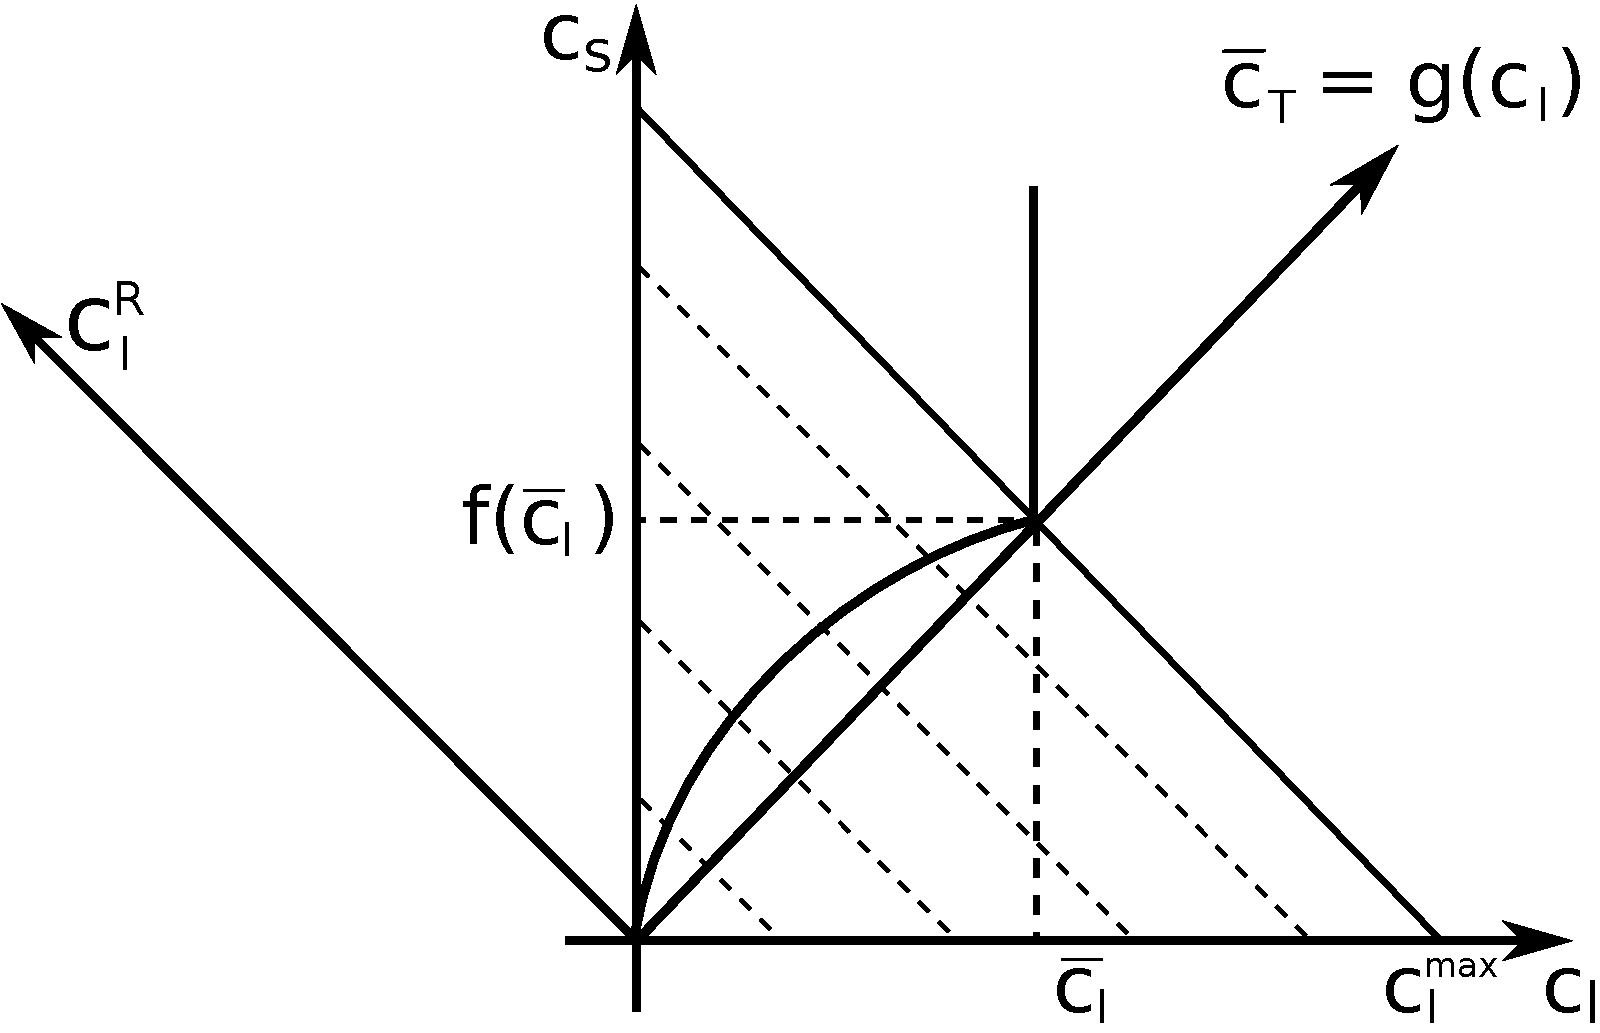
\includegraphics[width = 0.75\textwidth]{\fig/sorpce.pdf}
 \caption{Sorption in combination with limited solubility.}
 \label{fig:sorpce}
\end{figure}


To approximate the equation \eqref{eq:nonlin_sorption} using interpolation, we need to prepare the set of values 
which represents $[c_l, f(c_l)]$, with $c_l$ equidistantly distributed in transformed (rotated and rescaled) 
coordination system at first. The construction process of the interpolation table follows.
\begin{enumerate}
 \item Maximal ``total mass'' $\bar{c}_T = \mu_l\cdot \bar{c}_l + \mu_s\cdot f(\bar{c}_l)$ is computed.
 \item Total mass step is derived $mass\_step = \bar{c}_T/n\_steps$. $n\_steps$ is the number of
       \hyperA{Sorption::substeps}{substeps}.
 \item Appropriate $c_T^j = (mass\_step\cdot j)/\mu_l,~j\in \{0,\ldots, n\_steps\}$ are computed. 
 \item The equations $\mu_l \cdot c_T^j = \mu_l\cdot c_l^j + \mu_s\cdot f(c_l^j)~j\in \{0,\ldots, n\_steps\}$ are solved 
       for $c_l^j$ as unknowns. The solution is the set of ordered couples (points) 
       $[c_l^j,f(c_l^j)],~j\in\{0,\ldots,n\_steps\}$.
\end{enumerate}
After the computation of $\{[c_l^j,f(c_l^j)]\}$, we transform these coordinates to the system where the total mass is 
an independent variable. This is done by multiplication of precomputed points using the transformation matrix ${\bf A}$:
\begin{equation}
 \begin{array}{l}
  \vec{c}\,^R = {\bf A}\cdot\vec{c}\\
  \left[\begin{array}{c} c_l^{R,j}\\ c_s^{R,j} \end{array}\right] = 
  \left[\begin{array}{cc}
    \vartheta\cdot \rho_w & M_s(1 - \vartheta)\rho_R\\
    -M_s(1 - \vartheta)\rho_R & \vartheta\cdot \rho_w
  \end{array}\right]\cdot
  \left[\begin{array}{c} c_l^j\\ c_s^j \end{array}\right]\\
  j\in\{0,\ldots,n\_steps\}
 \end{array}
 \label{eq:transf_mat}
\end{equation}

The values $c_l^{R,j}$ are equidistantly distributed and there is no reason to save them, but the values 
$c_s^{R,j}$ are stored in onedimensional interpolation table.

Once we have the interpolation table, we can use it for projecting the transport results ${[c_l,c_s]}$ on the 
isotherm under consideration. Following steps must be taken.
\begin{enumerate}
 \item Achieved concentrations are transformed to the coordinate system through multiplication with the 
       matrix ${\bf A}$, see \eqref{eq:transf_mat}.
 \item Transformed values are interpolated.
 \item The result of interpolation is transformed back. The backward transformation consists of multiplication 
       with ${\bf A}^T$ which is followed by rescaling the result. Rescaling the result is necessary because  
       ${\bf A}$ is not orthonormal as it is shown bellow.
 \[
 \begin{array}{l}
 {\bf A}^T\cdot{\bf A} =
  \left((\vartheta - 1)^2\cdot M_s^2\cdot \rho_R^2 + \vartheta^2\cdot \rho_w^2\right)\cdot\left[\begin{array}{cc}
    1 & 0\\
    0 & 1
  \end{array}\right]
  \end{array}
 \]
\end{enumerate}


% \subsection{Limited Solubility}\label{subsec:lim_solub}
\paragraph{Limited solubility.} When $\mu_l\cdot c_l + \mu_s\cdot f(c_l) > \mu_l\cdot \bar{c}_l + \mu_s\cdot f(\bar{c}_l)$, neither iterative 
solver nor interpolation table is used. The aqueous concentration is set to be $\bar{c}_l$ and sorbed 
concentration is computed $c_s = (\mu_l\cdot c_l + \mu_s\cdot f(c_l) - \mu_l\cdot \bar{c}_l)/\mu_s$.

\subsection{System of Linear Ordinary Differential Equations}
\label{sec:num_slode}

A system of linear ordinary differential equations (ODE) appears in several places in the model. We provide 
several \hyperA{IT::LinearODESolver}{solvers} which we shall brielfy describe in this section. Let us denote 
the ODE system
\[
  \partial_t \vc c(t) = \mathbf{A}(t) \vc{c}(t) + \vc{b}(t).
\]

\paragraph{Semi-analytic solution.}
A \hyperA{IT::LinearODEAnalytic}{semi-analytic} solution can be obtained in special cases due to the physical nature of the problem.
The problem can be then solved only by a~matrix multiplication $\vc c(t+\Delta t) = \mathbf{R} \vc{c}(t)$. 
This is used in case of radioactive decays and first order kinetic reactions.

The right hand side $\vc{b}$ is zero and $\mathbf{A}$ is constant. The assumption is made that the equations 
are independent during one time step. Each quantity $c_i$ (concentration in this case) is decreased 
by $e^{a_{ii} \Delta t}$ (supposing negative diagonal) during time step $\Delta t$. The decrement $\left( 1-e^{a_{ii} \Delta t} \right)$
is then distributed among other quantities according to the given fraction.

In case of radioactive decays and first order reactions, the elements of the solution matrix $\mathbf{R}$ are
\begin{eqnarray*}
     r_{ii} &=& e^{-k_i \Delta t}, \\
     r_{ji} &=& \left( 1-e^{-k_i \Delta t} \right) b_{ji} \frac{M_j}{M_i},
\end{eqnarray*}
where $b_{ji}$ is the branching ratio of $i$-th reactant (or radionuclide) and $\frac{M_j}{M_i}$ is 
the fraction of molar masses.
The expressions $b_{ji} \frac{M_j}{M_i}$ are then obtained from the system matrix by dividing 
$-\frac{a_{ji}}{a_{ii}}$. See the system matrix entries in \eqref{eqn:reaction_system_entries}.

The assumption (equations independence) is adequate when a very small time step is applied. This will then lead 
to huge amount of evaluations of the exponential functions which can be expensive, so other numerical methods 
might be more appropriate. When the time step is large then the assumption is inadequate.

On the other hand, if the time step is constant (for significantly large number of time steps), we get the
solution cheaply just by matrix multiplication, because the matrix $\mathbf{R}$ is constant.


\paragraph{Pad{\' e} approximant.}
For homogenous systems with constant matrix $\mathbf{A}$, we can use \hyperA{IT::PadeApproximant}{Pad{\' e} approximation} 
to find the solution. This method finds a rational function whose power series agrees with a power series expansion of 
a given function to the highest possible order (e.g. in \cite{press_numerical_1992}).
Let
\[
  f(t) = \sum\limits_{j=0}^{\infty} c_j t^j = \sum\limits_{j=0}^{\infty} \frac{1}{n!}f^{(j)}(t_0)
\]
be the function being approximated and its power series given by Taylor expansion about $t_0$.
Then the rational function
\begin{equation} \label{eqn:pade_approximant}
R_{mn}(t) = \frac{P_m(t)}{Q_n(t)} = \frac{\sum\limits_{j=0}^{m} p_jt^j}{\sum\limits_{j=0}^{n} q_jt^j},
\end{equation}
which satisfies 
\begin{equation} \label{eqn:pade_coef_equations}
f(t)\approx \sum\limits_{j=0}^{m+n} c_j t^j = R_{mn}(t),
\end{equation}
% \begin{equation} \label{eqn:pade_coef_equations}
% \sum\limits_{j=0}^{m+n} c_jt^j \sum\limits_{j=0}^{m} q_jt^j = \sum\limits_{j=0}^{n} p_jt^j,
% \end{equation}
is called Pad{\' e} approximant. From \eqref{eqn:pade_coef_equations}, we obtain $m+n+2$ equations for
coefficients of the nominator $P_m$ (polynomial of \hyperA{PadeApproximant::nominator-degree}{degree} $m$) and 
the denominator $Q_n$ (polynomial of \hyperA{PadeApproximant::denominator-degree}{degree} $n$). We also see that the error 
of the approximation is $O(t^{m+n+1})$. By convention, the denominator is normalized such that $q_0=1$.

Now, we consider the solution of our ODE system in a form $\vc{c}(t)=e^{\mathbf{A}t}\vc{c}(0)$. We shall 
approximate the matrix exponential function using a matrix form of \eqref{eqn:pade_approximant}. 
For exponential functions, there are known coeffficients of the nominator and denominator:
% http://mathoverflow.net/questions/41226/pade-approximant-to-exponential-function
% http://www.math.vanderbilt.edu/~esaff/texts/144.pdf
% https://www-sop.inria.fr/apics/anap03/PadeTalk.pdf
\begin{eqnarray}
  \mathbf{P}_m(\mathbf{A}t) &=& \sum\limits^{m}_{j=0}\frac{(m+n-j)!m!}{(m+n)!j!(m-j)!} (\mathbf{A}t)^j, \\
  \mathbf{Q}_n(\mathbf{A}t) &=& \sum\limits^{n}_{j=0} (-1)^j \frac{(m+n-j)!n!}{(m+n)!j!(n-j)!} (\mathbf{A}t)^j.
\end{eqnarray}
Finally, we can write the solution at time $t+\Delta t$
\begin{equation} \label{eqn:pade_solution}
\vc{c}(t+\Delta t) = \frac{\mathbf{P}_m(\mathbf{A}\Delta t)} {\mathbf{Q}_n(\mathbf{A}\Delta t)}\vc{c}(t) 
= \mathbf{R}_{mn}(\mathbf{A}\Delta t)\vc{c}(t).
\end{equation}

If the time step $\Delta t$ is constant, we do not need to compute the matrix $\mathbf{R}_{mn}$ repeatedly and we get
the solution cheaply just by matrix multiplication. In the oposite case, we avoid evaluating the exponential
function and still get the solution quite fast (comparing to computing semi-analytic solution).